\documentclass[11pt]{book}
\usepackage{geometry}        
\geometry{letterpaper}    
\usepackage[parfill]{parskip}  
\usepackage{graphicx}
\usepackage{caption}
\usepackage{subcaption}
\usepackage{amssymb}
\usepackage{epstopdf}
\usepackage{listings}
\usepackage{times}

\usepackage[final]{pdfpages}


\DeclareGraphicsRule{.tif}{png}{.png}{`convert #1 `dirname #1`/`basename #1 .tif`.png}

\usepackage[colorlinks=true, pdfstartview=FitV, linkcolor=black, 
            citecolor=blue, urlcolor=blue]{hyperref}

\usepackage{tocloft}



\renewcommand\cftchapfont{\Large\bfseries}
\renewcommand\cftsecfont{\Large\bfseries}

%\renewcommand\cftchappagefont{\LARGE\bfseries}
%\renewcommand\cftsecpagefont{\LARGE}

\renewcommand\cftchapafterpnum{\par\addvspace{6pt}}
\renewcommand\cftsecafterpnum{\par\addvspace{6pt}}

% ------------------- Title and Author -----------------------------

\setlength\parindent{24pt}
\renewcommand{\baselinestretch}{1}
\linespread{1.5}

\begin{document}

\begin{titlepage}
    \begin{center}
                
        \Large
        \textbf{Intro Stat Shiny}
        
      
        \vspace{1cm}
       
        
        \Large
        Chelsey Legacy \\
        \vspace{0.25cm}
        Department of Statistics\\
          \vspace{0.25cm}
        Iowa State University\\
       
        
        \vspace{1cm}
               
           Creative Component\\
             \vspace{0.25cm}
           Spring 2017
           
           \vspace{2cm}
           
           Committee Members: Amy G. Froelich, Major Professor \\
              \vspace{0.25cm}
           \hspace{2.4cm} W. Robert Stephenson \\
              \vspace{0.25cm}
          \hspace{1cm} Heike Hofmann  
               
        
        
    \end{center}
\end{titlepage}







\begin{center}
\textbf{Abstract}
\end{center}
\newpage
\tableofcontents
\renewcommand\thechapter{\arabic{chapter}}
\renewcommand\thesection{\arabic{section}}
%\renewcommand\thesubsection{(\arabic{subsection})}

\newpage
\section{Introduction}
Technology has become an integral part of teaching undergraduate statistics courses. A lot of research has gone into the role technology can play in statistics courses and the positive affect  it can have on learning introductory statistics concepts.  R's Shiny applications create an easy to use interactive interface for users, which make them a great platform for introductory statistics students to use.  For these reasons a Shiny web application in addition to supplemental worksheets were created in order to aid student comprehension of the concepts of sampling distributions for one and two means, sampling distributions for one and two proportions, linear regression, and ANOVA analysis.   In this paper we will discuss the literature surrounding technology in statistics courses and outline the creation of an R shiny app and supporting supplemental worksheets to be used in conjunction with the app. 


\section{Literature Review}

	   
	   	
	Most undergraduate statistics courses make use of some sort of technology in the classroom from calculators to computer software programs.  All the available technology has the ability to simplify complex calculations in addition to making conceptual ideas more concrete.  These are two main features of technology that has helped make it a staple tool for statistics education.  Roy D. Pea provides an argument about why the computer as a cognitive technology is so important to the advancement in learning mathematics, in his article \emph{Cognitive Technologies for Mathematics Education} (1987).  Though his article focuses on the role of technology in math education there is a direct tie to statistics, in that he is discussing calculations and graphing data, both of which are essential elements of statistics courses.  He introduces cognitive technologies as ``any medium that helps transcend the limitations of the mind (e.g. attention to goals, short-term memory span), in thinking, learning, and problem-solving activities" (91). Computer applets and software are precisely the type of cognitive technologies being described that can help student thinking to go beyond just following formulas and returning answers.  
		
	  Pea goes on to describe this idea further,  ``a common feature to all these cognitive technologies is that they make external the intermediate products of thinking (e.g. output of the component steps in solving a complex algebraic equation), which can then be analyzed, reflected upon, and discussed" (Pea, 1987, p. 91).  With the help of computers, we are able to put thoughts and equations into visual and graphical representations that can then be viewed by many and discussed in an effort to clarify statistical concepts.  The main goal of this project was to be used in helping statistics students gain some insight and confidence in working with complex concepts.  Pea perfectly sums up this idea by saying that ``the dynamic and interactive media provided by computer software make gaining an intuitive understanding (traditionally the province of the professional mathematician) of the interrelationships among graphic, equational, and pictorial representations more accessible to the software user."(1987, p. 96)  Technologies such as R's Shiny web applications have the ability to provide insights to students through their interactivity and the output they provide that are not available through lectures or notes on a blackboard.
	 

The use of these technologies in the curriculum had a profound impact on the pedagogy of statistics. Chance et al. provide a discussion in  \emph{The Role of Technology in Improving Student Learning of Statistics} about how courses are changing format.  They specify that, "students are evaluated less on their ability to manipulate formulas and look up critical values, and more on their ability to select appropriate tools (e.g., choosing techniques based on the variables involved), assess the validity of different techniques, utilize graphical tools for exploration of data, deal with messier data sets, provide appropriate interpretations of computer output, and evaluate and communicate the legitimacy of their conclusions`` (p. 3).  They state, "technology has expanded the range of graphical and visualization techniques to provide powerful new ways to assist students in exploring and analyzing data and thinking about statistical ideas, allowing them to focus on interpretation of results and understanding concepts rather than computational mechanics`` (p. 3).    Though, technology has all the aforementioned benefits it is important that the technology should support the course learning objectives, and not restructure the objectives to pertain to learning the software.  Chance et al, argue that technology should not be used " merely for the sake of using technology",  but instead used for accessing, analyzing and interpreting large real data sets, automating calculations and processes, generating and modifying appropriate statistical graphics and models, performing simulations to illustrate abstract concepts and exploring 'what happens if...' type questions" (p.2-3).

There are increasingly many different software programs and applets available to supplement introductory statistics courses.  Chance et al describe how " the types of technology used in statistics and probability instruction can be broken into several categories: Statistical software packages, educational software, spreadsheets, applets/standalone applications, graphing calculators, multimedia materials, and data repositories." (p.4) These options all have advantages and drawbacks highlighted in the article by Chance et al.  


Choosing among these various options largely depends on the content of your course, your students expected competency on such programs, and funding available.  Fathom, Minitab, and JMP are all point and click programs that allow users to enter and manipulate data, and they will provide graphical and summary statistics of the data.  The drawback of such programs is that they cost the institution or the students money for downloads of the software.  Of course R and R studio can also provide the graphical output and summary statistics needed by the students and they are available for free.  However, with both R and the point and click software there is a learning curve for the students.    Many students may enter the course with little to no programming or even basic computer skills.   To avoid the course becoming inaccessible to those students, the software chosen should be fairly straightforward and require no previous knowledge.   Use of complex programs provides the problem of the students focusing so much on learning the software that they lose sight of the statistical concepts they are actually supposed to be learning.  

 In addition to software, there are many great web based java applets that are free to use and provide conceptual frameworks for simulations, p-values, and other intro stat concepts made available by Rossman and Chance (2004).  These are helpful additions to already created lecture slides and materials, however they do not provide any supplemental materials that can help guide student interaction with the applets.  As pointed out by Doi et al in \emph{Web Application Teaching Tools for Statistics Using R and Shiny}, there are a multitude of available software and programs, however eventually an instructor may have difficulty finding an applet or software that perfectly suits their needs for their lectures (p. 1).
 
 With monetary and time costs to consider, R`s Shiny app technology is a great option for technology to incorporate into the classroom.  R`s package allows the developer to create an interactive app that is point and click based, and allows the user to perform complex tasks with the click of a button.  In Doi et al's article the authors provide a discussion on the advantages of using Shiny in the classroom. One of the main advantages is that the user never has to engage in writing or seeing the code if the developer chooses.  The developer is the only one that must have a basic understanding of coding in R to get the app successfully running (p. 6, Doi et al, 2016).
 The authors explain that, "all adjustments in the app are done by moving sliders or clicking buttons and corresponding updates to the output plot are virtually instantaneous. This leads to a much more fluid and dynamic presentation." (p. 6). After creation and publication to the web the app can be run from a web browser so students can easily interact with it.  Apps can be made for a variety of topics for the course and accessed from phones, tablets, and computers.  This also allows the technology to be used by all students in classrooms other than just computer classrooms, which is appealing to lectures without access to computer classrooms.

 In addition, Doi et al discuss how the ease of design of a Shiny app allows it to be "especially helpful when teaching concepts that are not in the standard curriculum or based on recent research" (p 6. 2016).  Newer concepts may not already have applets or software available for classroom demonstrations, thus Shiny can be used to create something to fills that gap.  It could also be used to create tailor made lecture materials for a specific course.  Apps can be created based on the different topics in that course and thus creating a collection of relevant tools for a corresponding course. 
 
 

\section{Shiny Web Application Design}
Designing and programming the R Shiny app for this project was a large part of this project. There are many different concepts introduced to students in introductory statistics courses.  A few of these concepts were chosen to be the focus of the shiny app.  The topics the shiny app provides materials and displays for are inference for one and two sample proportions, inference for one and two means, linear regression topics, and ANOVA.  The web application is composed of several tabs each dedicated to one of these topics.Using the Shiny reference and examples pages a design was planned out for each of the different sections. Then, the applications were programmed for each section and subsection. 

\begin{figure}
        \centering
        \quad
        \begin{subfigure}[b]{0.5\textwidth}
                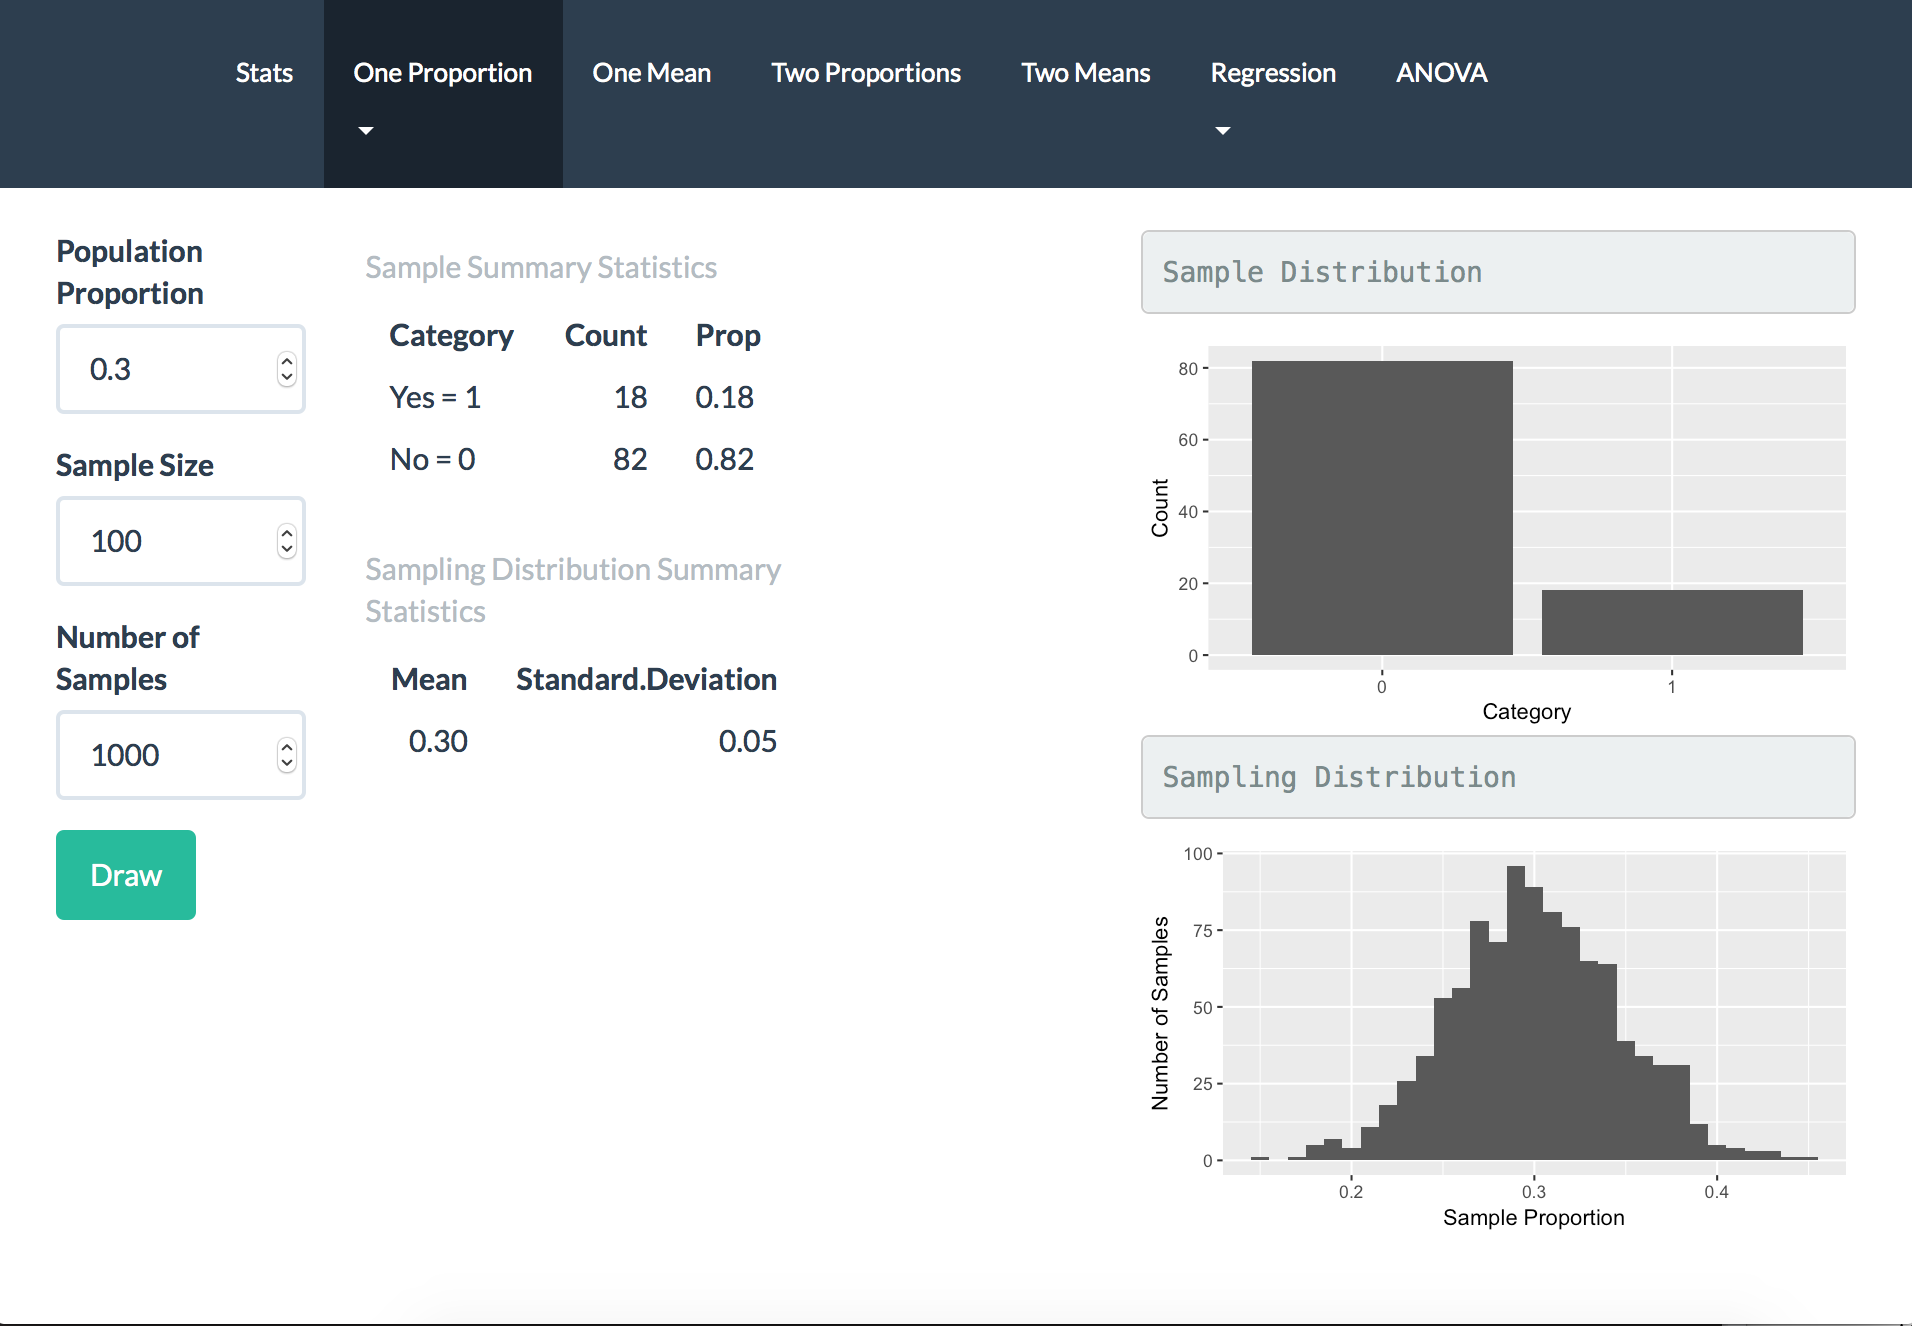
\includegraphics[width=\textwidth]{OneProp.png}
                \caption{Sampling Distribution Screen }
                \label{fig:OneProp}
        \end{subfigure}%
	\quad
        \begin{subfigure}[b]{0.5\textwidth}
                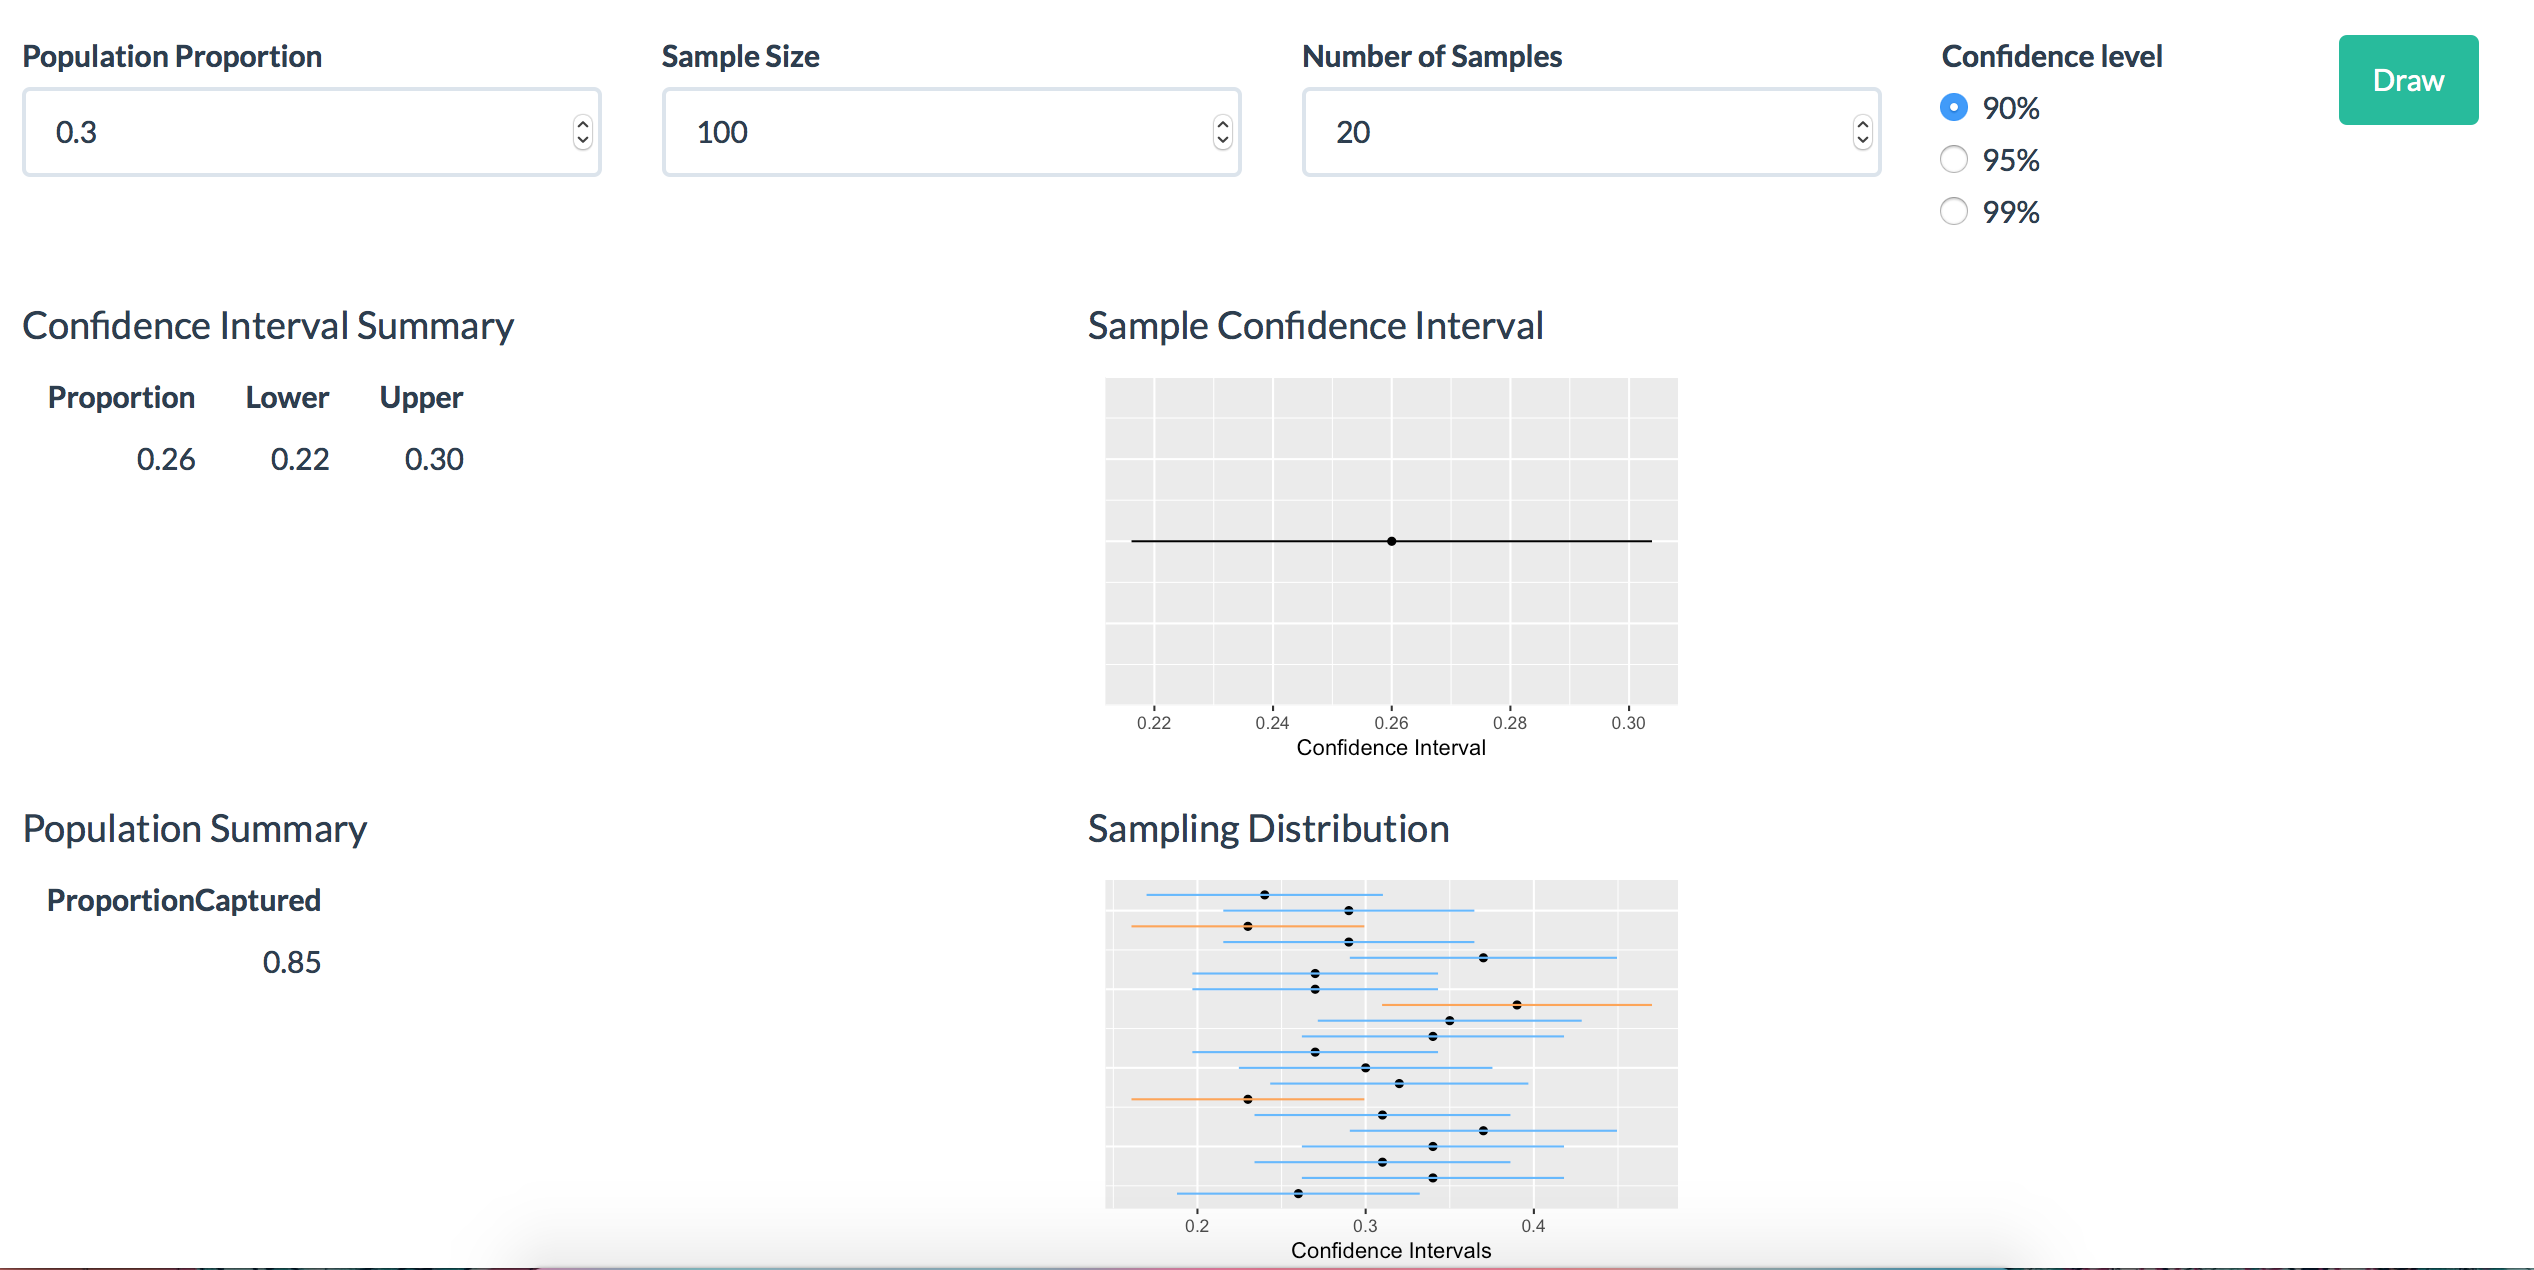
\includegraphics[width=\textwidth]{OnePropCL.png}
                \caption{Confidence Level Screen} 
                \label{fig:OnePropCL}
        \end{subfigure}
	\quad
        \begin{subfigure}[b]{0.5\textwidth}
                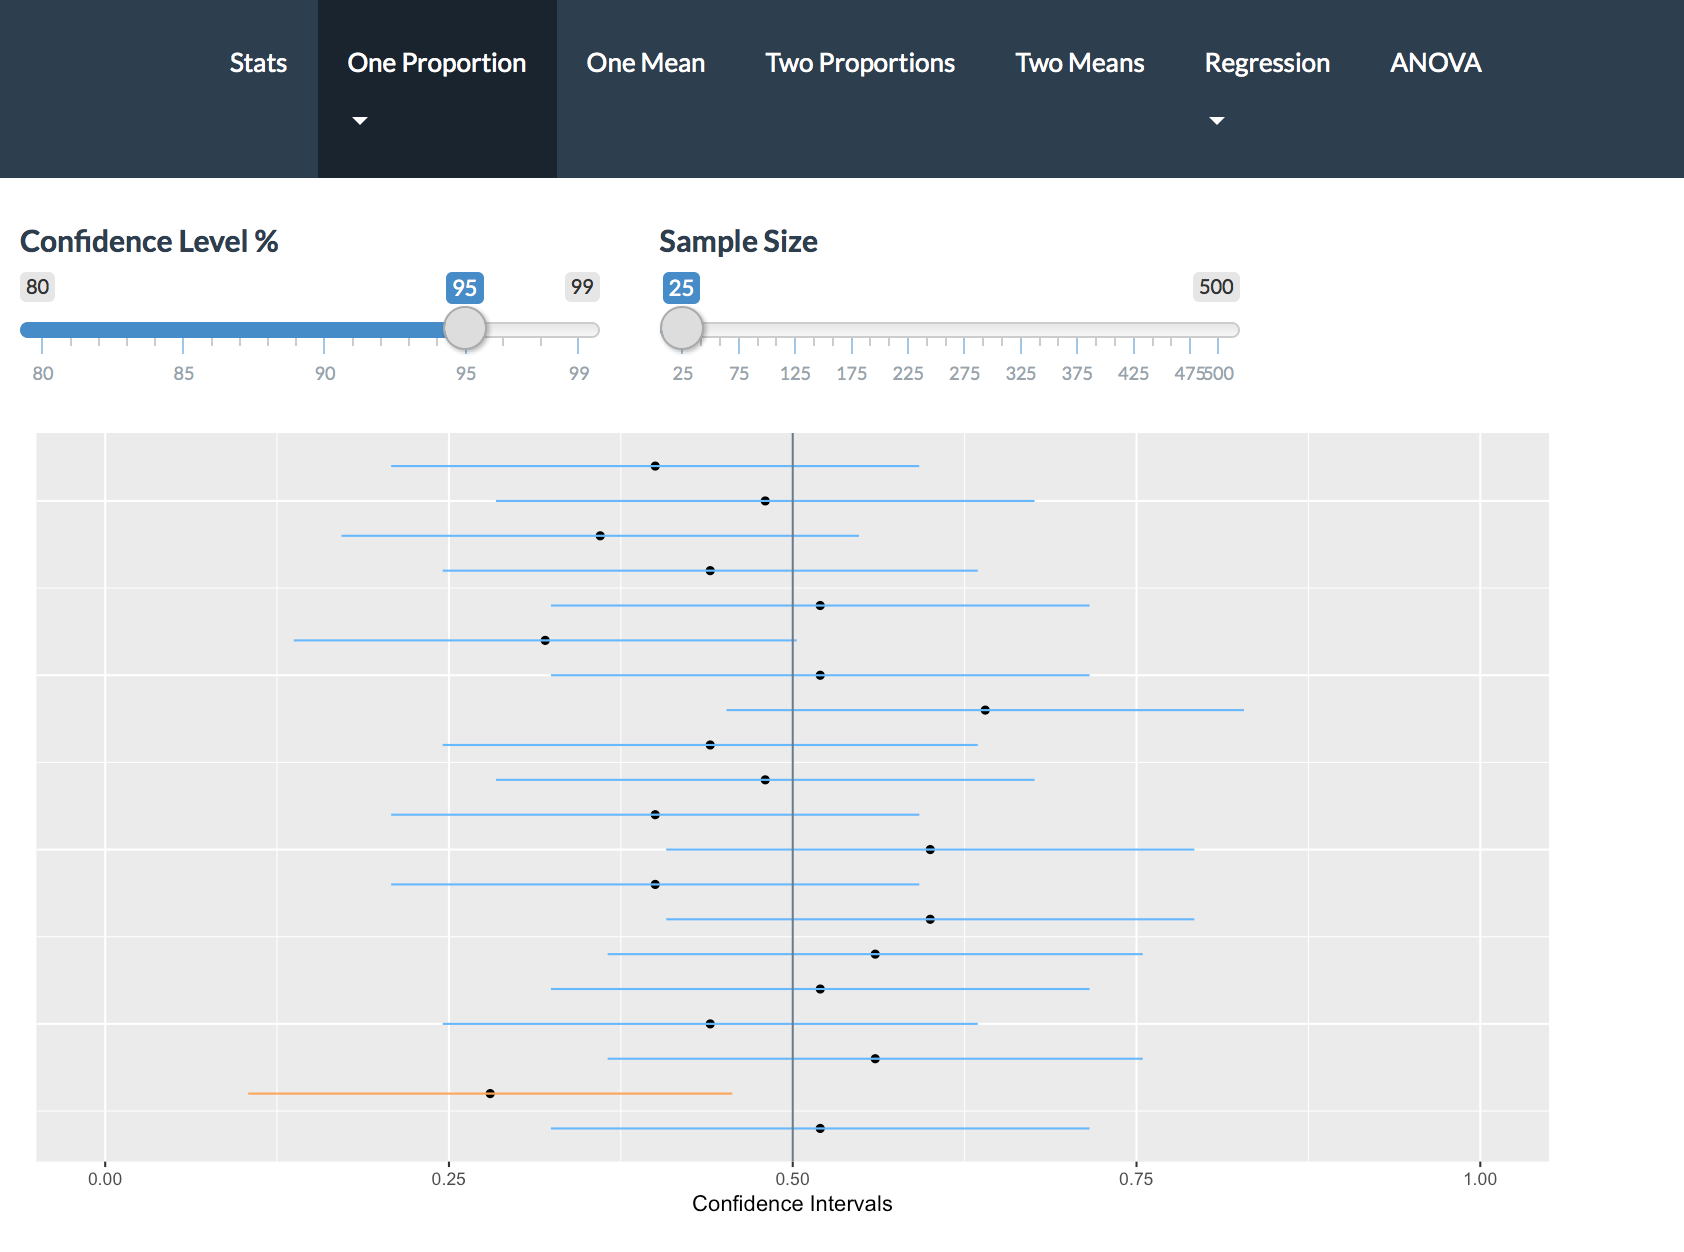
\includegraphics[width=\textwidth]{OnePropCI.png}
                \caption{Confidence Interval Screen } 
                \label{fig:OnePropCI}
        \end{subfigure}
	\quad
        \begin{subfigure}[b]{0.5\textwidth}
                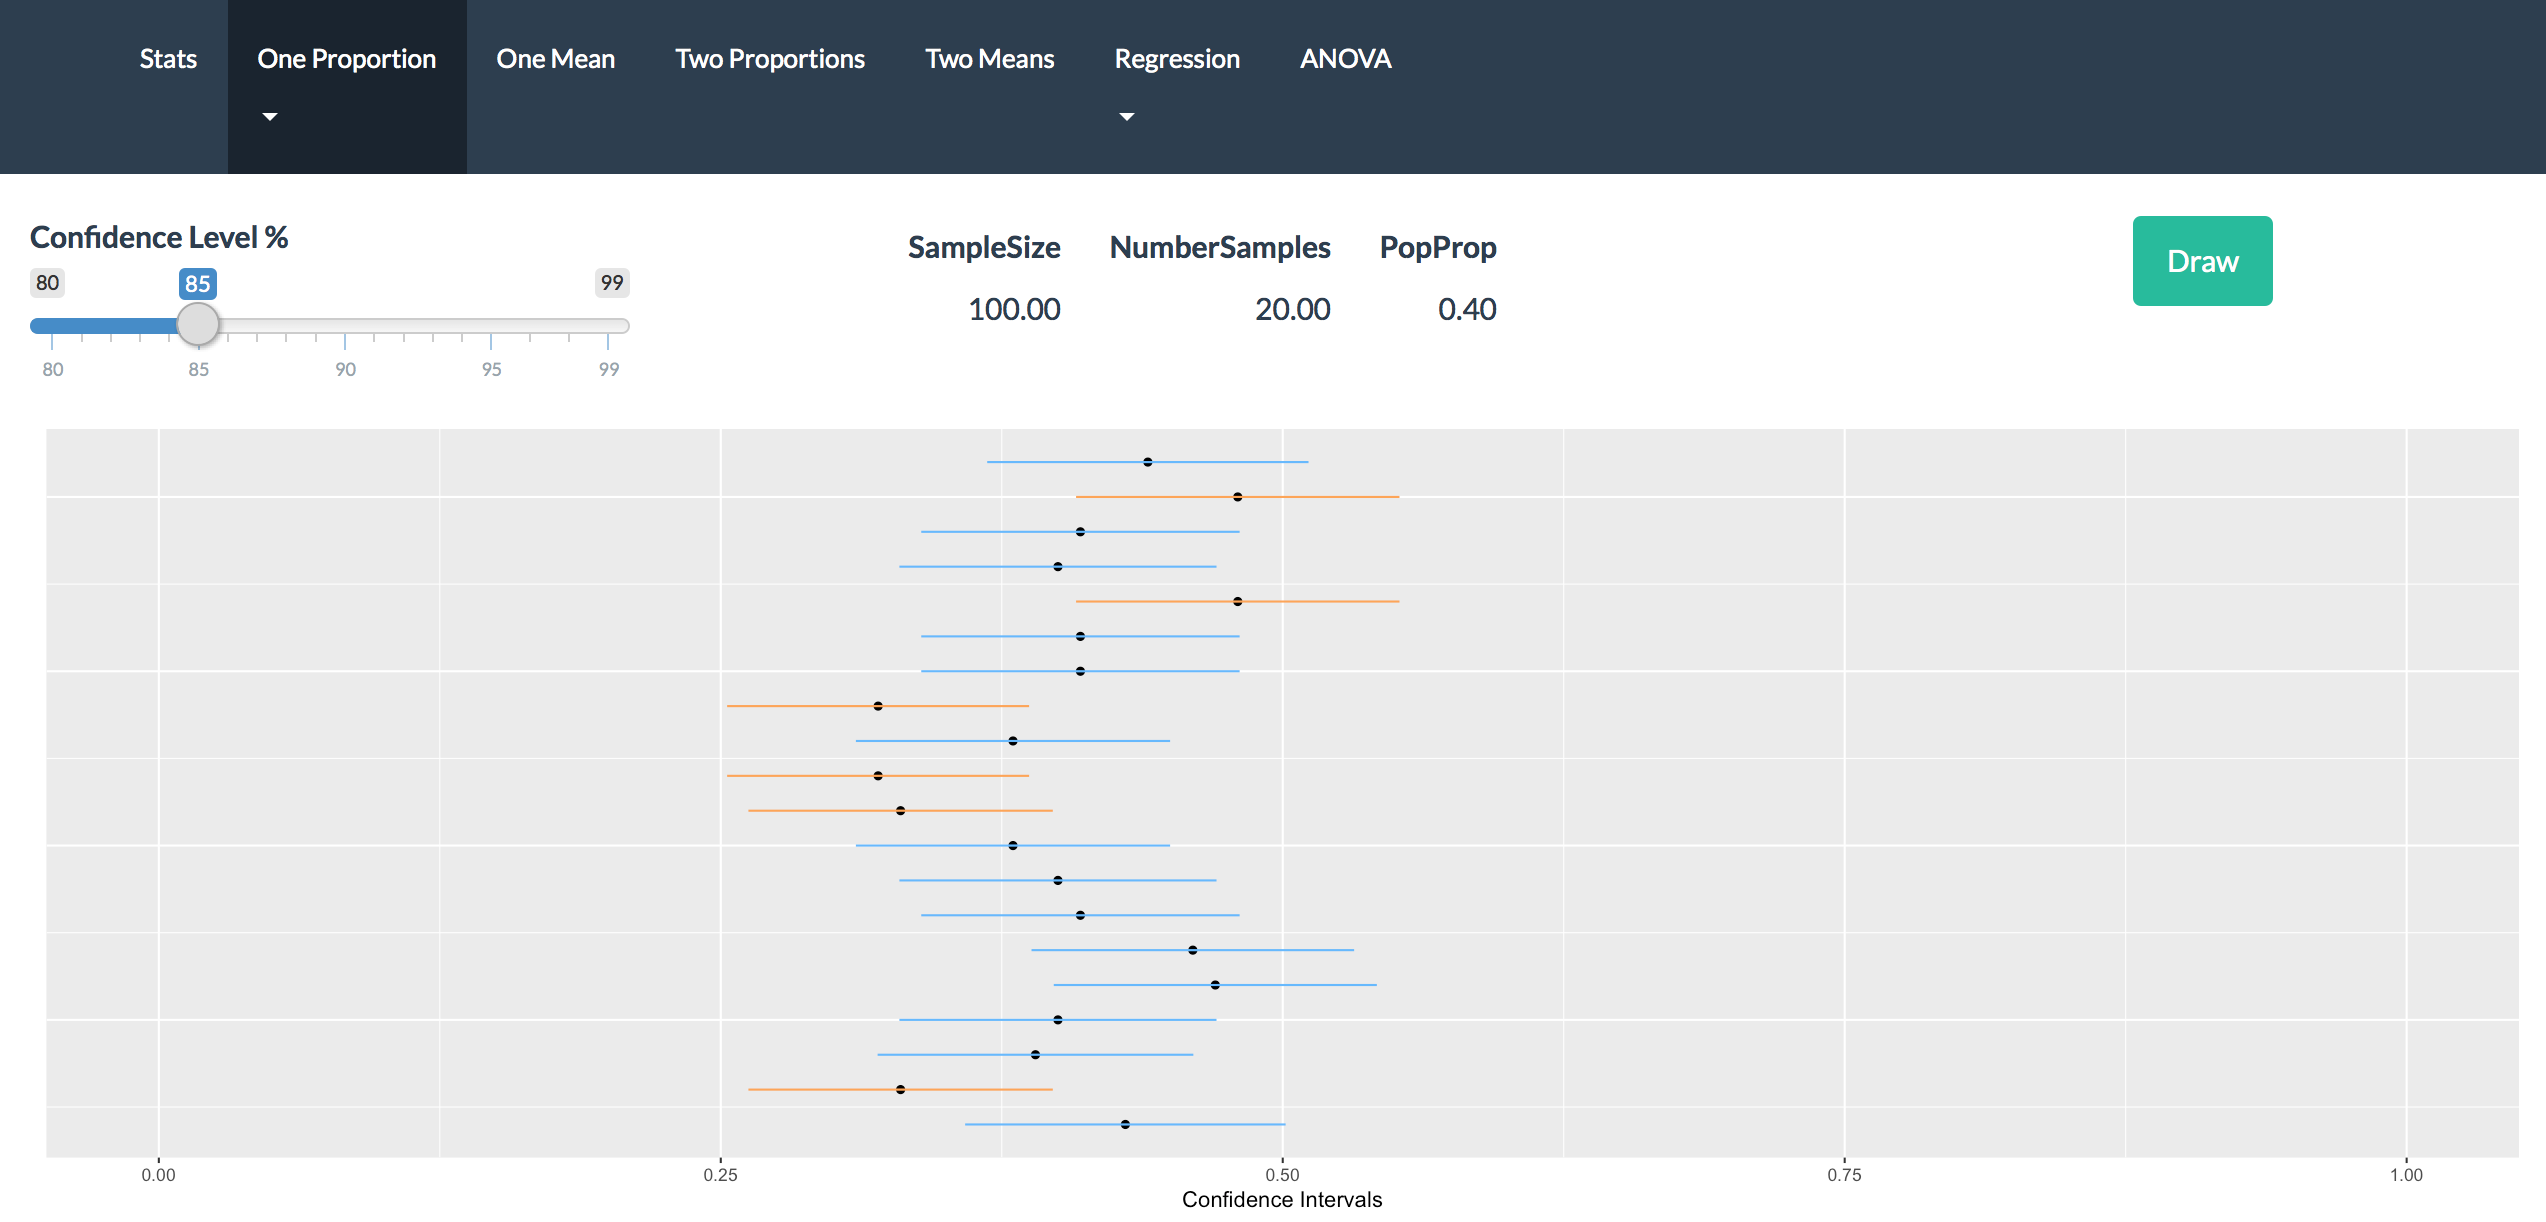
\includegraphics[width=\textwidth]{OnePropSampSize.png}
                \caption{Sample Size Screen}
                \label{fig:OnePropSampSize}
        \end{subfigure}%
	
\label{AllWeather}
\caption {All the subsections of Inference for One Proportion.}
\end{figure}

As seen in Figure~\ref{OneProp} the Shiny application opens up to the sampling distribution for one sample proportion.  There are several other topics that pertain to the inference for one proportion that become available once the "Inference for One Proportion" tab is clicked.  The entire collection of topics for the inference for one proportion include, sampling distribution, confidence interval, sample size, and confidence level.   The design for this topic was based on the design of several JMP scripts currently used in Statistics 101 at Iowa State University.  This section is designed to help enhance student comprehension of the difference between a sample distribution and sampling distribution for a sample proportion.  At the top of the application a variety of variables such as sample size, number of samples, and population proportion can be manipulated.  Once these are set to the desired amounts the user can hit the draw button and the application will perform the simulation.  The middle graph and chart represent the sample distribution and sample summary information for the last sample drawn.  The bottom section chart and graph represent the population of all samples drawn.  The samples are drawn from a binomial with mean specified by the user inputs.  The worksheet that corresponds to this section leads student through drawing one sample and seeing how it is displayed in the the sample distribution vs in the sampling distribution. Then the students are led to draw more samples and see that the sampling distribution ends up centered around population proportion.  The Figure~\ref{OneProp} shows a sample display once many samples have been drawn.

 


The next section under the inference for one proportion is designed to demonstrate the construction of confidence intervals. A screen shot of this section can be found in Figure~\ref{OnePropCL} The top boxes allow user inputs of the population proportion, sample size, number of samples, and confidence level.  The middle section displays the upper and lower bound for a randomly selected sample proportion based on the user set inputs above. The graph shows the interval for the last selected sample.  The bottom output shows the interval for each sample chosen for each sample size.  A blue interval indicates that the confidence interval captured the true population proportion set by the user.  An orange interval indicates that the interval did not capture the population proportion.  In the population summary you can see what proportion of the intervals created around the samples proportions captured the true population proportion.  In the worksheet the students are asked to investigate how the proportion captured will more closely match the confidence level as the sample size increases.  

Another important concept for inference for one proportion is the idea of how sampling size affects the confidence interval, which is why a section was created just for this concept.  It is possible to observe this with the section just on confidence intervals, but for further emphasis this section was created. Figure~\ref{OnePropSampSize} shows that for this section the number of samples, population proportion and confidence level are all fixed quantities.  The only quantity available for manipulation is the sample size.  Similar to the section on confidence intervals the graph displays a confidence interval.  As the user slides the sample size bar to larger sample sizes it is easy to see that the interval  gets  smaller.  The worksheet corresponding to this section has the students investigate this in order to come to the conclusion that as sample size increases that the width of the confidence interval will decrease.


The final subsection for inference for one proportion, shown in Figure~\ref{OnePropCL}, is on the effect of confidence level on confidence intervals.  This section is similar to the one before it, but here the sample size, number of samples, and population proportion are all fixed.  The slider allows the user to manipulate the confidence level and see its effect on the size of the confidence interval.  As the slider increases the confidence level from 80 to 99 percent we can see that the confidence intervals get larger and there are more intervals that capture the true population proportion.  The students are led through this idea in the corresponding worksheet.   

Another section featured in the shiny application is  about linear regression topics.  There are separate pages designed to help aid the learning of correlation and linear regression.  The correlation page features a slider that allows the user to select correlation values for a random plot of points.  This allows the user to see what different correlations look like ranging from -1 to 1.  The linear regression section allows the user to either look at fitting lines to a plot of preloaded sample data, or look at fitting a line to a group of points.  This section allows the user to input the slope and intercept they desire, then the data will be generated based on what was selected.  A line can then be fit to the specifications the user wanted.  This allows the user to see the relationship between the slope, intercept and the data points that they choose.  

The next section featured focuses on the concept of sampling distribution for one mean. They layout is similar to that of the inference for one proportion sampling distribution.  The top inputs allow the user to enter the mean, standard deviation, sample size, and number of samples.  Once the "Draw" button is clicked the sampling distribution begins to appear with summary statistics in addition to the last drawn sample distribution and its summary statistics.   Similar to the one proportion inference, the worksheet for this section walks the student through taking multiple samples to build the sampling distribution which ends up being approximately normal.

Next, there are sections for each, sampling distributions for the difference in sample proportions and the difference in sample means for two groups.  These sections have a similar layout as the previous sections for obtaining sampling distributions.  The user inputs the necessary information for each of the two groups at the top of the screen.  The middle graphs display the sample distributions of each of the two samples.  Then, the bottom graphs display the sampling distribution of the differences between the two groups.  The user is also able to do a test for the difference in the groups.  They can select a one or two tailed test and will be given the corresponding p-vlaue.  


\begin{figure}
\centering
      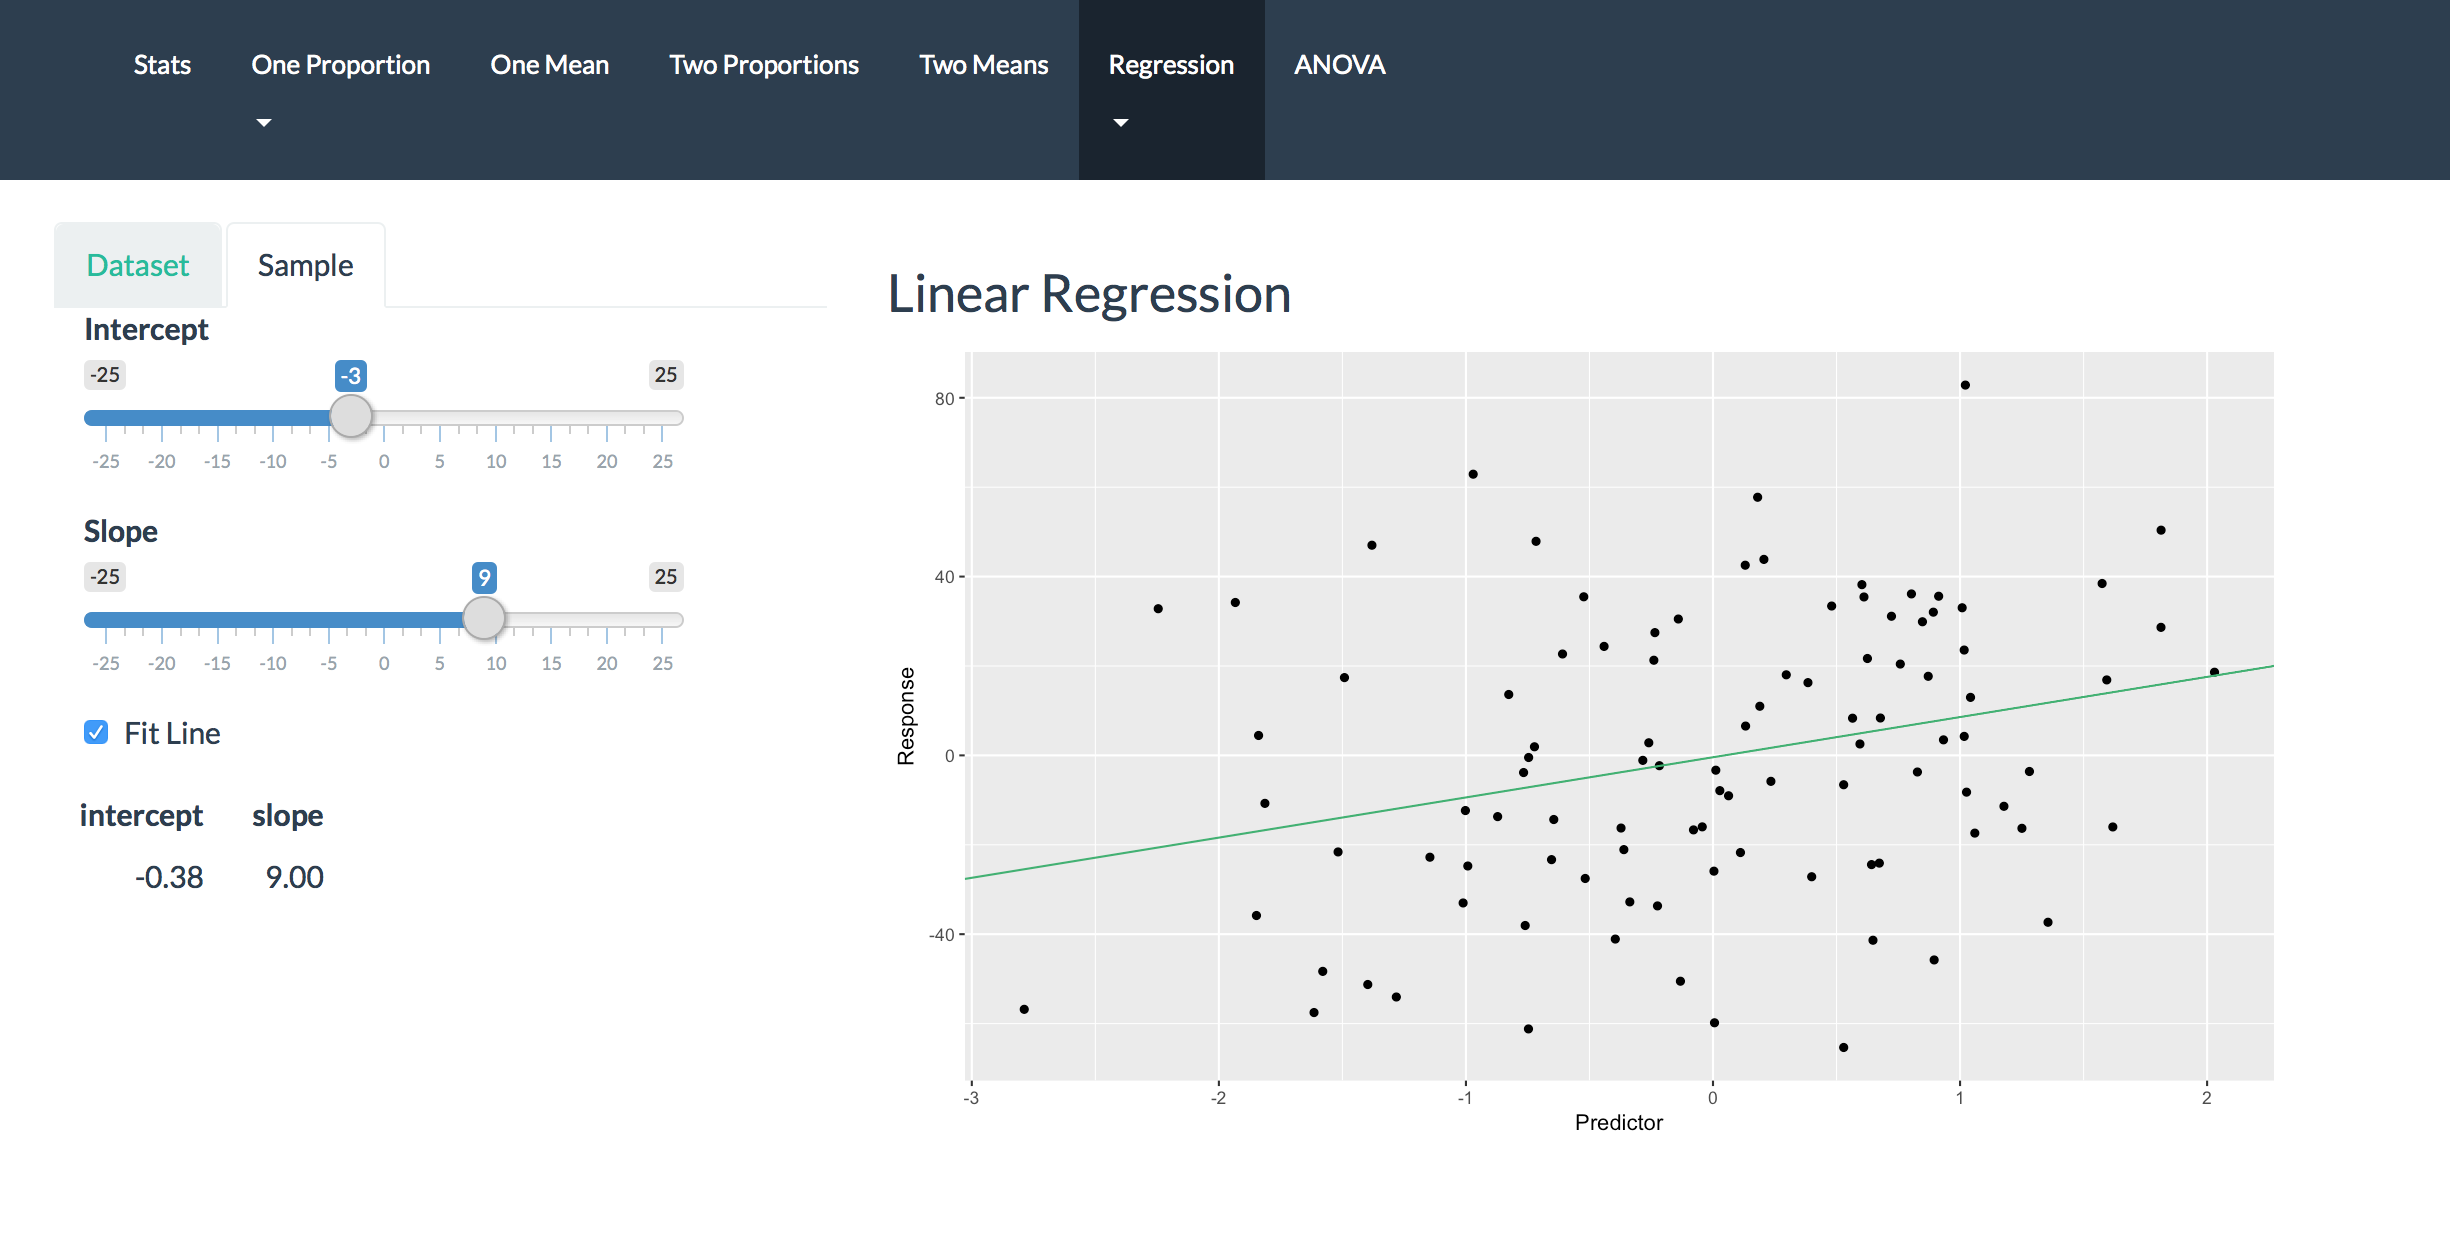
\includegraphics[width=\textwidth]{LinReg.png}
\end{figure}


The tab for Linear Regression contains both basic linear regression plots in addition to a section on exploring correlation.  The tab for linear regression shown in Figure~\ref{LinReg} allows the user to select a preloaded data set and add a line of best fit.  The data will be plot on a scatterplot with the line of best fit, and the output of the line formula will be shown.  The corresponding worksheet asks the user to identify and interpret the different parts of the equation for the line.  In the Linear Regression tab the user can also randomly generate data corresponding to a specific set of user input specifications.  The user can input a slope and intercept and the corresponding data will be plotted on the scatterplot.  This section allows the user to explore how changing the intercept affects the lines placement, in addition to how changing the sign of the slope affects the direction of the points and the line of best fit.  

\begin{figure}
\centering
        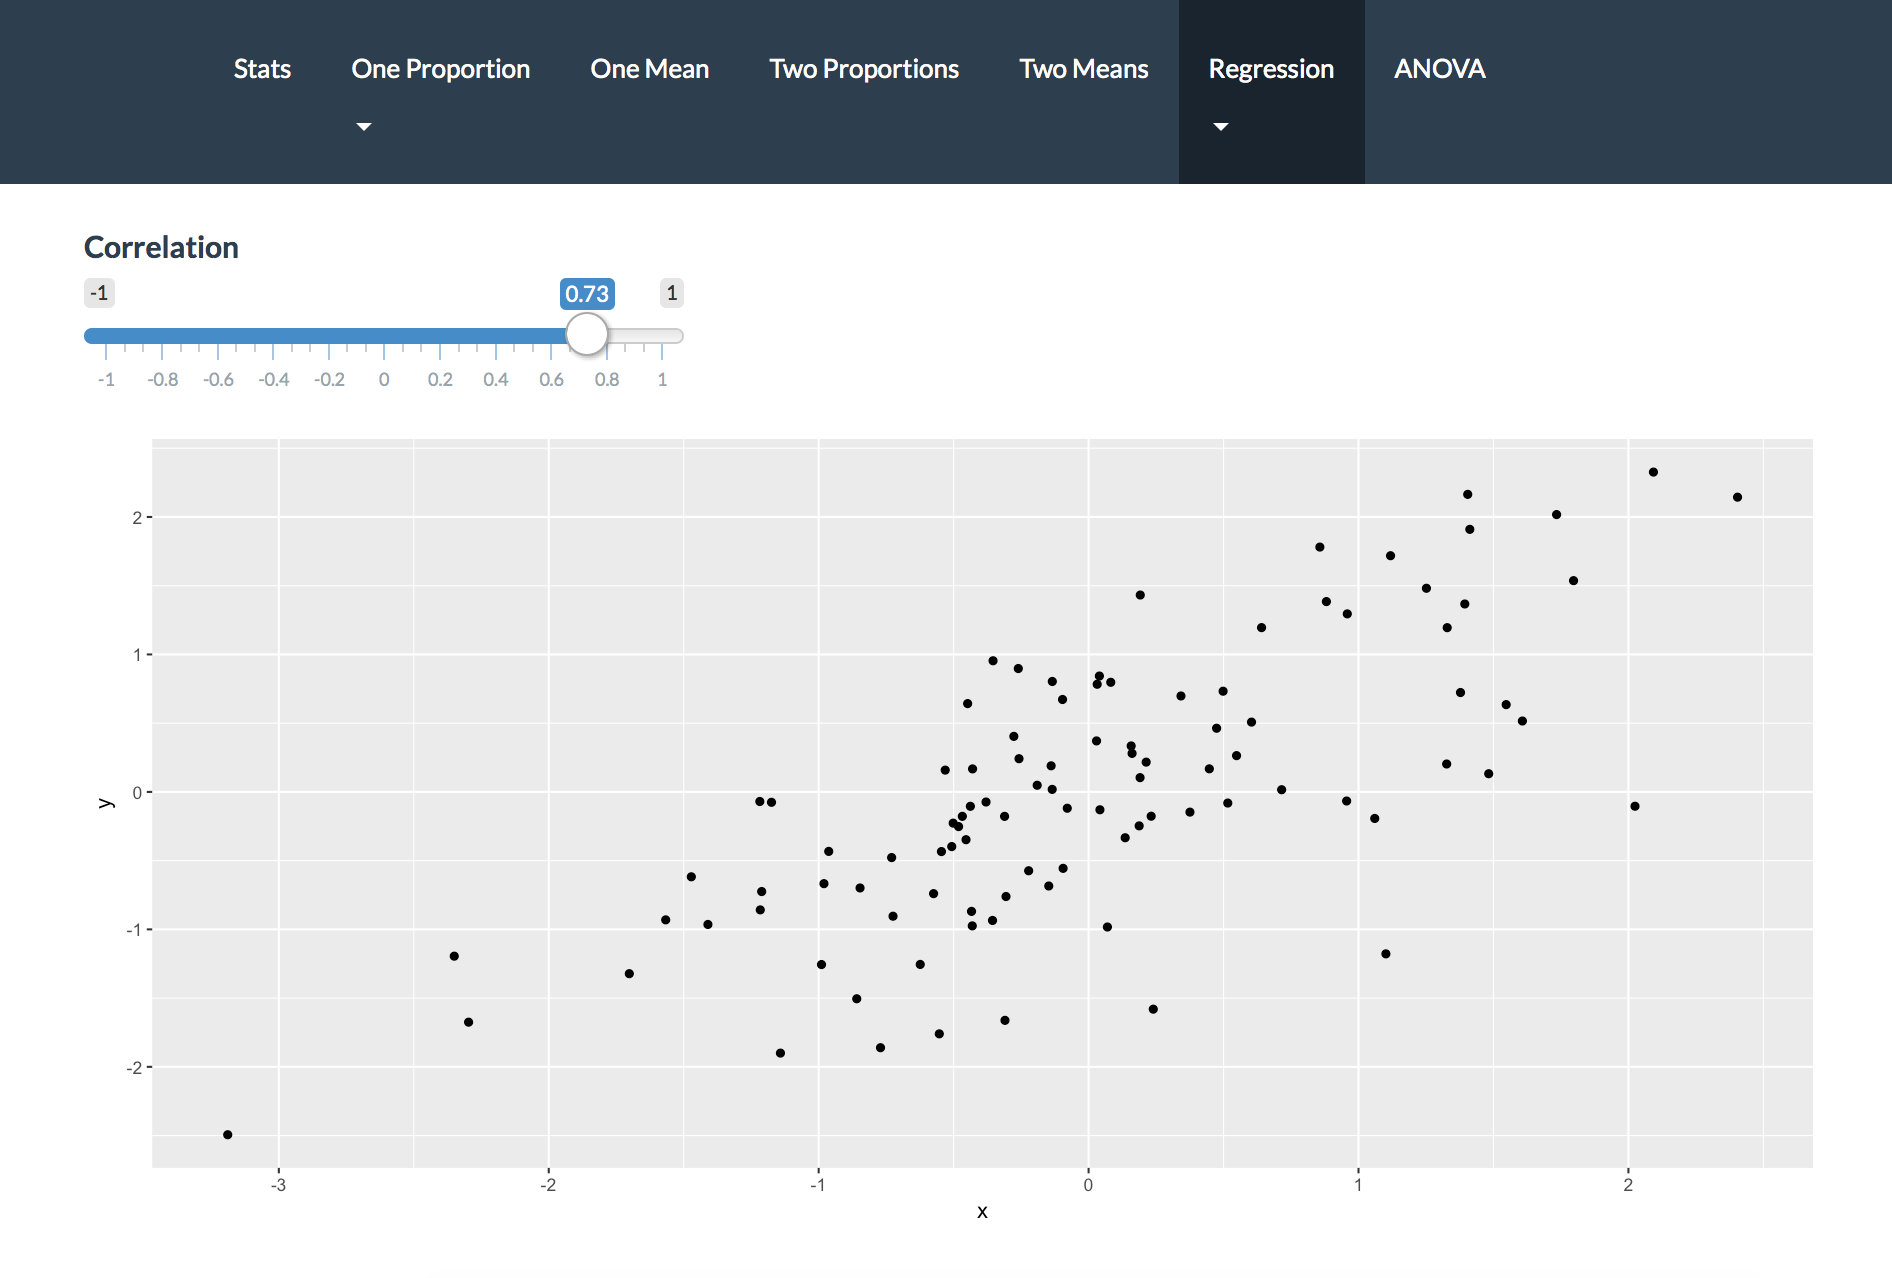
\includegraphics[width=\textwidth]{Correlation.png}
\end{figure}




The correlation section of this tab allows the user to manipulate a slider with range from -1 to 1.  The slider corresponds to the correlation of points on a scatterplot below.  From this, the user can see the relationship between different levels of correlation and what the corresponding graphs will look like.  



The last tab of the shiny application is the ANOVA tab.  This tab explores the relationship among the means of 3 different groups.  The user can input the means, standard deviations, and sample sizes for each of the three groups.  Then the middle graph will display a dotplot for each group.  Below the graph is an ANOVA table for the differences in the means along with the summary information for each of the three groups.  The corresponding worksheet gives the student a small introduction to the ANOVA F test followed by some questions asking them to explore the relationship between the mean, standard deviation, sample size and the resulting p-value and conclusion to the F-test. 
\section{Experimental Design}
\section{Implementation}
\section{Testing}


\section{Discussion}
\section{Conclusion}
\section{References}


 \begin{thebibliography}{1}

\bibitem{chance}  Chance, B., Ben-Zvi, D.,$\&$ Garfield, J.,  Medina, E. (2007). The Role of Technology in Improving Student Learning of Statistics.

\bibitem{doi}  Doi, J., Potter G., Wong J., Alcaraz I., $\&$ Chi, P. (2016). Web Application Teaching Tools for Statistics Using R and Shiny. 

\bibitem{Pea} Roy D. Pea. Cognitive Technologies for Mathematics Education. A. Schoenfeld. Cognitive science and mathematics education. Hillsdale, pp.89-122, 1987. $<$hal-001990547$>$

\bibitem{Rossman} Rossman, A.$\&$ Chance, B. (2004), The \emph{Rossman/Chance Applet Collection}. Available at www.rossmanchance.com/applets.


  \end{thebibliography}

\section{Appendix}

\subsection{Worksheets}

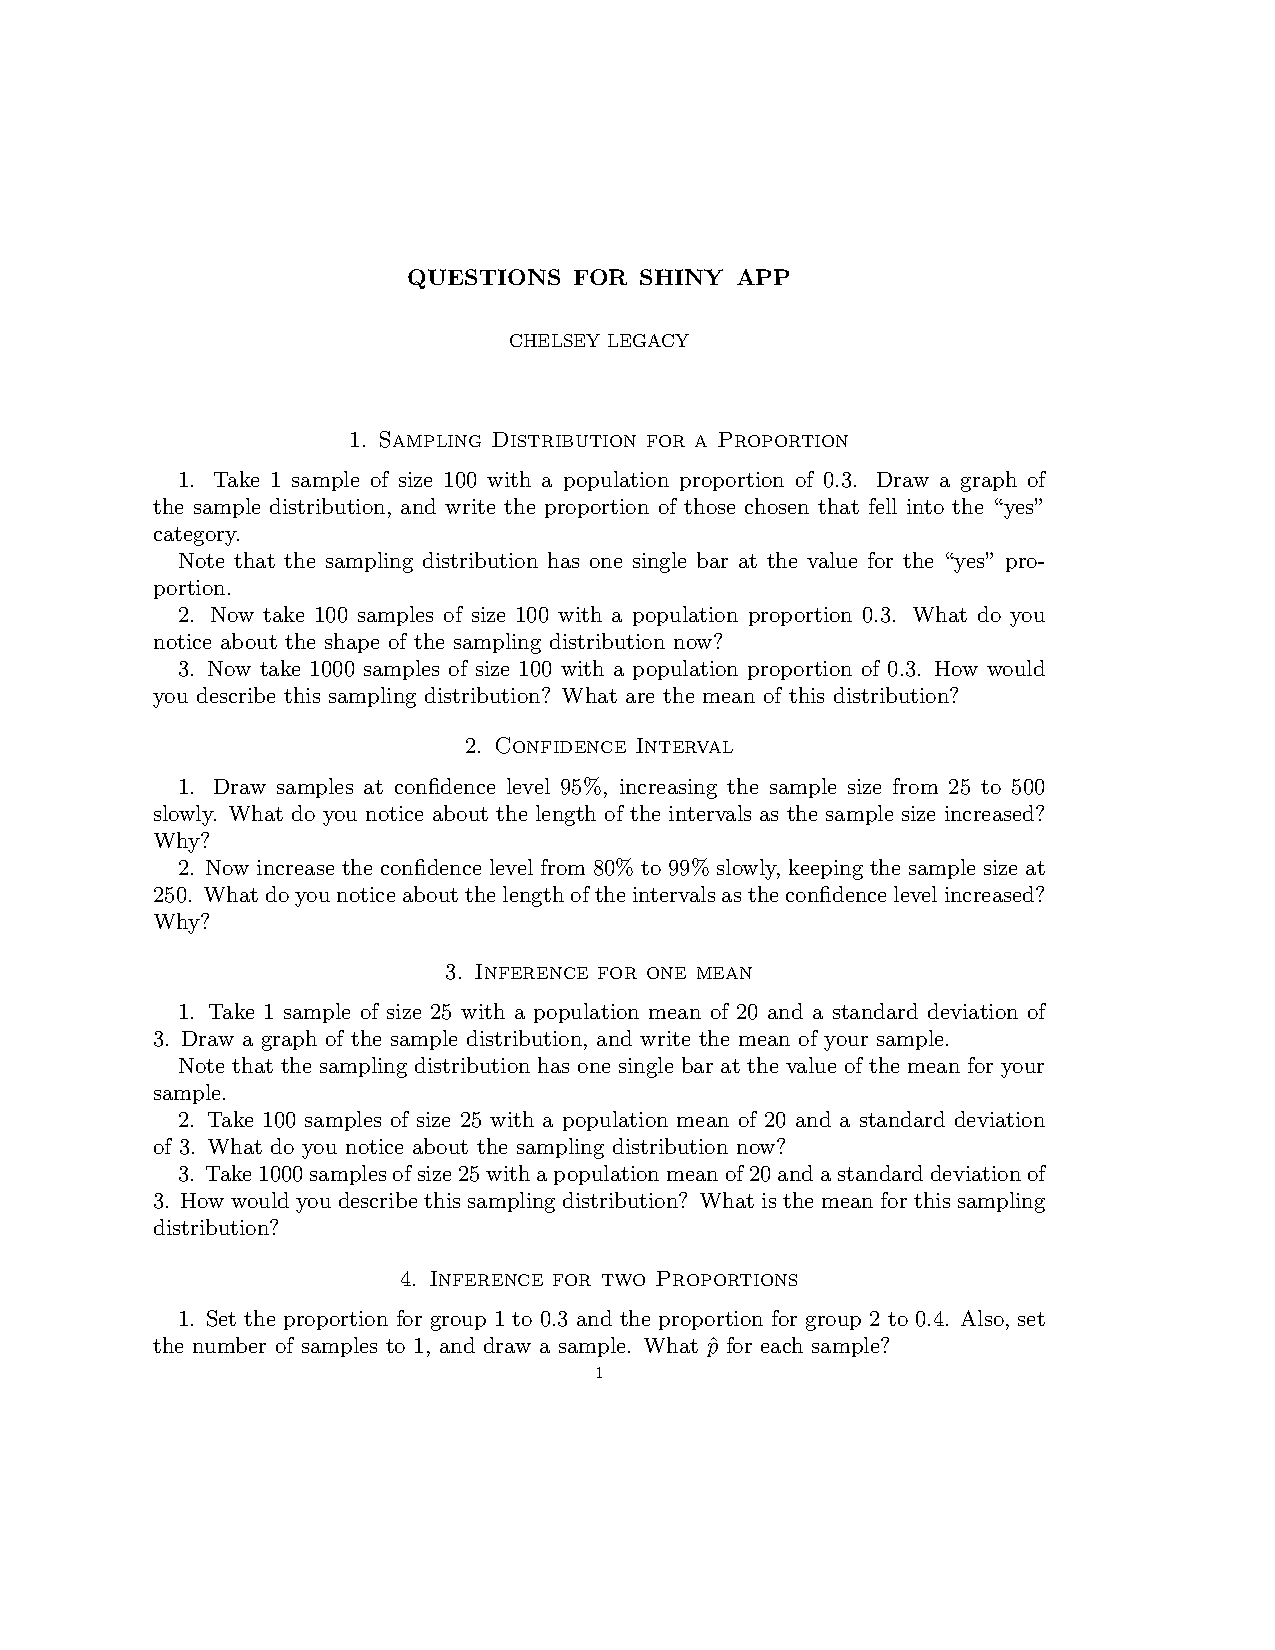
\includepdf[pages=-]{Questions.pdf}








\end{document}
\end

